% !TeX program = pdflatex
% UTF-8; all experiments below are synthetic compilation fixtures.
\documentclass[UTF8,a4paper,12pt]{ctexart}
\usepackage{amsmath,amssymb,graphicx,booktabs,geometry,longtable}
\geometry{margin=25mm}
\setlength{\parindent}{2em}
\setlength{\parskip}{0.3em}
\renewcommand{\arraystretch}{1.15}
\title{面向离线文档系统的合成传感器异常检测实验\\\large 多文件中文论文与参考文献编译验证样例}
\author{LightOverLeaf 测试工作组\\\small 软件功能验证用稿，非真实科研成果}
\date{2026 年 9 月}
\begin{document}
\maketitle
\begin{abstract}
为验证本地 LaTeX 编辑器对中文正文、数学表达、长表格、位图和参考文献的完整支持，本文构建一个可复算的合成传感器异常检测实验。研究对象为 120 个按确定性规则生成的观测点，比较固定阈值、保守残差阈值和灵敏残差阈值三种规则。通过统一的混淆矩阵和准确率、精确率、召回率及 F1 指标呈现检测差异，并提供全部逐点数据和图片生成脚本。本文的贡献是形成具有数据一致性约束的编译验证材料，而非证明某一算法在真实工业环境中的优势。所有数据均为人工合成，三条参考文献对应随项目提供的内部测试说明，不代表已发表研究。
\end{abstract}
\noindent\textbf{关键词：}离线编辑器；合成数据；异常检测；参考文献；编译验证
\clearpage
\tableofcontents
\clearpage
\section{引言}
\label{sec:introduction}
本地论文编辑器不仅需要正确显示文本，还需要协调多文件输入、编译中间文件、参考文献辅助程序和 PDF 预览。一份仅有标题和一段文字的文档，难以暴露交叉引用未收敛、图片未被复制到快照或参考文献未生成等问题。因此，测试输入应具有接近论文的结构，同时使每一个数值和引用都可以追踪。

本样例选择传感器异常检测作为叙述载体。周期性温度序列具有直观的物理类比，阈值方法易于表达为公式，也能自然产生曲线图、混淆矩阵及指标表。这里的“温度”只是测试单位，不来源于真实传感器。数据集编号为 LOL-SYN-120，生成约定见内部测试说明\cite{lolData2026}。

本文围绕三个问题组织实验：第一，固定阈值与残差阈值在含周期项的序列上呈现何种差异；第二，阈值降低是否伴随误报与漏报的变化；第三，数据、表格、图片和引用能否在离线环境中组成可重复编译的论文。前两个问题只在本合成序列内讨论，第三个问题才是项目的主要验收目标。

\subsection{相关工作与引用边界}
为了避免将虚构文献包装为真实学术来源，本文仅引用三个本地内部测试记录。数据协议\cite{lolData2026}定义生成公式与标签；指标说明\cite{lolMetrics2026}固定混淆矩阵方向及舍入规则；复现指南\cite{lolReproduce2026}描述脚本、文件结构及编译顺序。这些条目用于验证 BibTeX 引用链路，不构成外部文献综述，也不能支持现实世界中的算法有效性结论。

\subsection{组织结构}
第\ref{sec:method}节定义数据和检测规则，第\ref{sec:experiment}节展示数值与图像，第\ref{sec:discussion}节讨论限制，附录提供全部观测记录。跨文件章节引用、表格引用及公式引用均由 LaTeX 自动编号，禁止手工写死页码和序号。

\section{方法与数据生成}
\label{sec:method}
\subsection{合成信号}
观测下标为 $i\in\{1,\ldots,120\}$，相邻观测间隔定义为 1 秒。周期基线、确定性扰动和标签分别为
\begin{align}
b_i &= 20+2\sin(i/8), \label{eq:baseline}\\
\epsilon_i &= 0.6\sin(1.7i),\\
y_i &= \begin{cases}1,& i\bmod 10=0,\\0,&\text{其他情况。}\end{cases}
\end{align}
在此基础上构造观测值
\begin{equation}
x_i=b_i+\epsilon_i+2y_i+1.6\mathbf{1}[i\bmod17=0].
\label{eq:signal}
\end{equation}
最后一项是人为设置的非目标扰动，不计入异常标签。因此，标签只由下标是否为 10 的倍数决定，而不是由幅度自动决定。它刻意模拟一个简化的“高幅度不一定属于目标异常”的测试场景。公式中的三角函数使用弧度，数据计算采用双精度，CSV 仅在输出时保留六位小数。

\subsection{对照检测器}
定义残差 $r_i=|x_i-b_i|$，三种检测器为
\begin{align}
\hat y_i^{(A)}&=\mathbf{1}[x_i>22],\\
\hat y_i^{(B)}&=\mathbf{1}[r_i>1.8],\\
\hat y_i^{(C)}&=\mathbf{1}[r_i>1.55].
\end{align}
A 为固定阈值基线，B 为保守残差规则，C 为较灵敏的残差规则。这里 B、C 直接使用已知生成基线，并未从训练集估计趋势；这是一项有意简化的先验优势，不能据此声称它们优于真实部署中的其他方法。

\subsection{评价指标}
按真实标签为行、预测标签为列排列混淆矩阵：
\begin{equation}
\mathbf{M}=\begin{bmatrix}\mathrm{TN}&\mathrm{FP}\\\mathrm{FN}&\mathrm{TP}\end{bmatrix}.
\end{equation}
指标定义如下，所有分母为零时约定对应指标为零\cite{lolMetrics2026}：
\begin{align}
\mathrm{Accuracy}&=\frac{\mathrm{TP}+\mathrm{TN}}{N},&
\mathrm{Precision}&=\frac{\mathrm{TP}}{\mathrm{TP}+\mathrm{FP}},\\
\mathrm{Recall}&=\frac{\mathrm{TP}}{\mathrm{TP}+\mathrm{FN}},&
F_1&=\frac{2\mathrm{TP}}{2\mathrm{TP}+\mathrm{FP}+\mathrm{FN}}.
\label{eq:f1}
\end{align}
准确率可能被多数类主导，因此本文同时报告四个指标而不只选择最大的数值。该数据只有一个固定生成实例，不计算没有抽样依据的置信区间，也不进行显著性检验。

\section{实验配置与结果}
\label{sec:experiment}
\subsection{配置及数据划分}
\begin{table}[htbp]\centering
\caption{确定性合成实验配置}\label{tab:config}
\begin{tabular}{ll}\toprule
项目 & 设置\\\midrule
样本总数 & 120\\
目标异常数 / 正常数 & 12 / 108\\
异常比例 & 10\%\\
周期基线 & 式\eqref{eq:baseline}\\
随机种子 & 不使用随机数\\
训练集 / 验证集 & 不适用，无学习过程\\
评估集 & 全部 120 个合成观测\\
固定阈值 / 残差阈值 & 22 / 1.8、1.55\\
统计精度 & 双精度计算，表格保留四位小数\\\bottomrule
\end{tabular}\end{table}
所有规则在生成数据之前即已固定，没有基于结果搜索最优阈值。为便于复现，生成脚本一次性写出原始数据、指标表、混淆矩阵、完整数据附录和两幅 PNG 图片。表格与图片消费同一份内存数据，避免手工复制数值造成不一致。

\subsection{时间序列可视化}
\begin{figure}[htbp]\centering
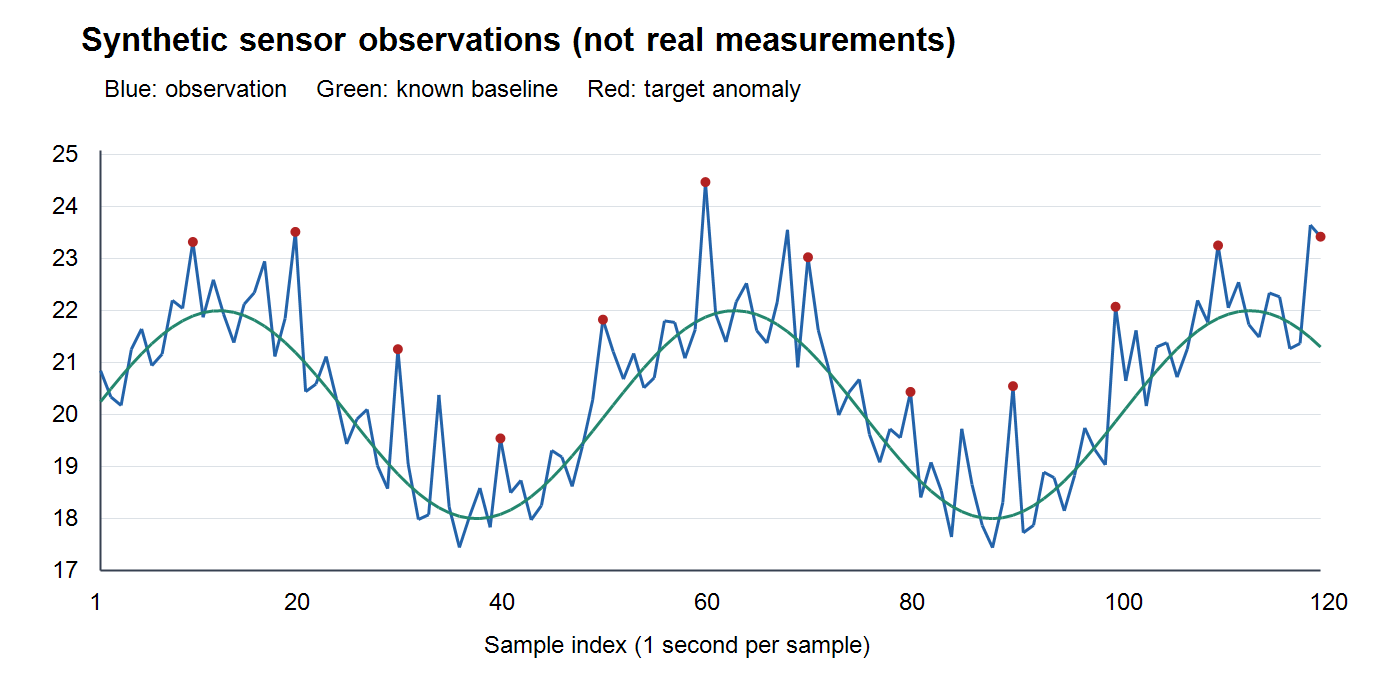
\includegraphics[width=0.96\linewidth]{figures/signal.png}
\caption{合成观测与已知基线。红点表示目标异常；横轴为样本下标，纵轴为合成温度。图片内英文标签用于避免绘图阶段依赖中文字体。}\label{fig:signal}
\end{figure}
图\ref{fig:signal}中的周期项使固定阈值在高基线区域更容易触发，在低基线区域则可能漏过目标异常。残差规则消除了已知周期项，但仍可能将非目标扰动判为异常。注意，“消除周期项”只是在公式已知的前提下相减，不涉及模型训练或实际信号分解。

\subsection{定量比较}
\begin{table}[htbp]\centering
\caption{合成数据上的检测指标}\label{tab:metrics}
\begin{tabular}{lrrrr}\toprule
规则 & Accuracy & Precision & Recall & $F_1$\\\midrule
A & 0.8250 & 0.3043 & 0.5833 & 0.4000\\
B & 0.9333 & 0.7000 & 0.5833 & 0.6364\\
C & 0.9333 & 0.6667 & 0.6667 & 0.6667\\
\bottomrule\end{tabular}\end{table}
\begin{table}[htbp]\centering
\caption{可独立复算的混淆矩阵计数}\label{tab:confusion}
\begin{tabular}{lrrrr}\toprule
规则 & TP & TN & FP & FN\\\midrule
A & 7 & 92 & 16 & 5\\
B & 7 & 105 & 3 & 5\\
C & 8 & 104 & 4 & 4\\
\bottomrule\end{tabular}\end{table}
表\ref{tab:metrics}使用式\eqref{eq:f1}等定义计算；表\ref{tab:confusion}给出全部整数计数，便于独立复算。每一行都必须满足 $\mathrm{TP}+\mathrm{FN}=12$、$\mathrm{TN}+\mathrm{FP}=108$，且四项计数之和为 120。

\begin{figure}[htbp]\centering
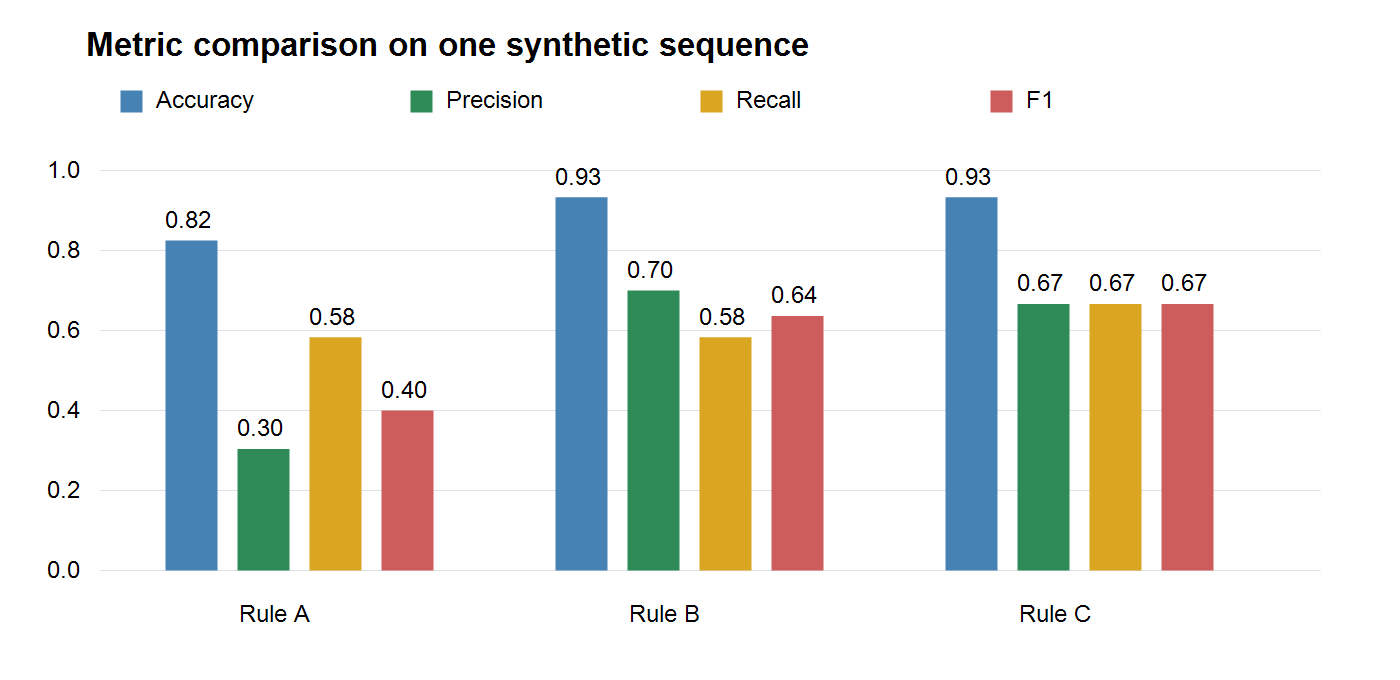
\includegraphics[width=0.86\linewidth]{figures/metrics.png}
\caption{三种检测规则的指标比较。数值范围为 0 至 1，与表\ref{tab:metrics}使用同一计算结果。}\label{fig:metrics}
\end{figure}
对 B 与 C 而言，降低阈值使预测正例集合只增不减，因此召回率不应下降，误报数也不应下降；精确率和 F1 则不保证单调。图\ref{fig:metrics}用于检查这种数值关系及图片嵌入是否正确，不用于替代逐点计数。

\subsection{可复算样本与错误分析}
\begin{table}[htbp]\centering\small
\caption{前十二个观测点}\label{tab:sample}
\begin{tabular}{rrrrrrrr}\toprule
$i$ & $b_i$ & $x_i$ & $r_i$ & $y_i$ & A & B & C\\\midrule
1 & 20.249 & 20.844 & 0.595 & 0 & 0 & 0 & 0\\
2 & 20.495 & 20.341 & 0.153 & 0 & 0 & 0 & 0\\
3 & 20.733 & 20.177 & 0.555 & 0 & 0 & 0 & 0\\
4 & 20.959 & 21.255 & 0.296 & 0 & 0 & 0 & 0\\
5 & 21.170 & 21.649 & 0.479 & 0 & 0 & 0 & 0\\
6 & 21.363 & 20.943 & 0.420 & 0 & 0 & 0 & 0\\
7 & 21.535 & 21.164 & 0.371 & 0 & 0 & 0 & 0\\
8 & 21.683 & 22.198 & 0.515 & 0 & 1 & 0 & 0\\
9 & 21.805 & 22.043 & 0.238 & 0 & 1 & 0 & 0\\
10 & 21.898 & 23.321 & 1.423 & 1 & 1 & 0 & 0\\
11 & 21.962 & 21.872 & 0.089 & 0 & 0 & 0 & 0\\
12 & 21.995 & 22.595 & 0.600 & 0 & 1 & 0 & 0\\
\bottomrule\end{tabular}\end{table}
表\ref{tab:sample}列出前十二个点，涵盖正常点和第一个目标异常。更详细的失败分析可在 CSV 中筛选 $y_i\ne\hat y_i$。对 A 应同时观察基线所处相位，对 B、C 应观察扰动叠加后的残差，不应把每次误报都解释为程序错误。

\subsection{编译与复现协议}
主文件为 \texttt{main.tex}，章节通过 \texttt{input} 组织，图片使用相对路径。首次排版后执行 BibTeX，再运行两轮 pdfLaTeX；目录、引用及参考文献稳定后才作为最终产物。编译全过程不需要网络、Shell Escape 或外部图片服务\cite{lolReproduce2026}。

\section{讨论、局限与结论}
\label{sec:discussion}
\subsection{有效性边界}
本实验是单变量、固定长度、确定性生成的评估场景。异常标签由生成协议规定，不来自独立专家标注。B 和 C 使用真实基线，因此它们在本样例中的表现不能直接外推到漂移、缺失、多变量或未知周期环境。更不能把这些合成指标当作设备故障识别的真实准确率。

表格中的六位数据和四位指标是显示精度，不代表测量精度；本样例没有真实测量误差模型。虽然附录包含 120 条记录，但它们不是 120 次独立随机试验，不能据此把标准误简单缩小为原来的 $1/\sqrt{120}$。

\subsection{文档系统的验收价值}
从软件角度看，成功生成 PDF 只是基础要求。还应检查：章节和目录编号是否一致，正文引用是否显示为问号，参考文献是否只有已引用的三条，PNG 是否清晰，跨页表格是否重复表头，以及修改数值后能否在下一次预览中看到变化。

故意删除图片、移除一个文献键或写错公式，可以作为错误定位测试，但这些破坏性场景应在副本中进行。默认交付文件保持可成功编译，不混入未闭合环境或不存在的资源。同步定位依赖编译器产生的 SyncTeX 文件，不能仅凭 PDF 页数推断其功能正常。

\subsection{结论}
本文给出了一套完整的中文多文件论文样例，将确定性数据生成、数学定义、三线表、长表格、图片和三条正文引用组合为可复现编译输入。样例的核心价值在于可核对、可重新生成且明确区分合成测试与真实研究。未来可以在独立副本中扩展长文档、大图片和复杂文献样式压力测试，但不应把额外宏包或外部工具悄悄加入当前离线依赖链。

\section*{数据声明与致谢}
全部数值、图像及内部测试文献由本样例生成或编写，不包含真实个人数据。作者署名为测试工作组，不对应真实学术机构。感谢本地编辑器提供编译验证环境；该表述不意味着任何第三方对实验结论背书。

\clearpage
\bibliographystyle{plain}
\bibliography{references}
\clearpage
\appendix
\section{功能验收清单}
\begin{longtable}{p{0.22\linewidth}p{0.68\linewidth}}
\toprule 功能 & 检查方法\\\midrule\endhead
中文正文 & 标题、摘要、段落和标点显示完整，无方框替代。\\
数学公式 & 检查矩阵、分段函数、上下标与对齐公式。\\
交叉引用 & 图、表、章节、公式编号不出现双问号。\\
图片资源 & 两张 PNG 都能显示，坐标轴和图例可辨识。\\
表格 & 指标表不越界，长表跨页时重复表头。\\
参考文献 & 正文三种引用键均解析，文末有三条内部测试记录。\\
多文件 & 修改方法章节后重新编译，更新出现在 PDF。\\
数据一致性 & CSV 总计 120 行，异常 12 个，三种混淆矩阵分别合计 120。\\
错误定位 & 在副本中故意写错一个命令，确认日志能够定位。\\
离线性 & 关闭网络后编译；不要启用宏包自动安装。\\\bottomrule
\end{longtable}

\section{全部逐点数据}
下表中的 A、B、C 分别对应三种规则，1 表示预测异常，0 表示正常。表中数值显示至三位小数，CSV 保留六位，判定使用未舍入值。
\small
\begin{longtable}{rrrrrrrr}
\caption{全部 120 条合成观测及预测}\label{tab:full}\\
\toprule $i$ & $b_i$ & $x_i$ & $r_i$ & $y_i$ & A & B & C\\\midrule\endfirsthead
\toprule $i$ & $b_i$ & $x_i$ & $r_i$ & $y_i$ & A & B & C\\\midrule\endhead
\midrule\multicolumn{8}{r}{续下页}\\\endfoot
\bottomrule\endlastfoot
1 & 20.249 & 20.844 & 0.595 & 0 & 0 & 0 & 0\\
2 & 20.495 & 20.341 & 0.153 & 0 & 0 & 0 & 0\\
3 & 20.733 & 20.177 & 0.555 & 0 & 0 & 0 & 0\\
4 & 20.959 & 21.255 & 0.296 & 0 & 0 & 0 & 0\\
5 & 21.170 & 21.649 & 0.479 & 0 & 0 & 0 & 0\\
6 & 21.363 & 20.943 & 0.420 & 0 & 0 & 0 & 0\\
7 & 21.535 & 21.164 & 0.371 & 0 & 0 & 0 & 0\\
8 & 21.683 & 22.198 & 0.515 & 0 & 1 & 0 & 0\\
9 & 21.805 & 22.043 & 0.238 & 0 & 1 & 0 & 0\\
10 & 21.898 & 23.321 & 1.423 & 1 & 1 & 0 & 0\\
11 & 21.962 & 21.872 & 0.089 & 0 & 0 & 0 & 0\\
12 & 21.995 & 22.595 & 0.600 & 0 & 1 & 0 & 0\\
13 & 21.997 & 21.932 & 0.065 & 0 & 0 & 0 & 0\\
14 & 21.968 & 21.385 & 0.583 & 0 & 0 & 0 & 0\\
15 & 21.908 & 22.124 & 0.215 & 0 & 1 & 0 & 0\\
16 & 21.819 & 22.346 & 0.528 & 0 & 1 & 0 & 0\\
17 & 21.701 & 22.949 & 1.249 & 0 & 1 & 0 & 0\\
18 & 21.556 & 21.119 & 0.437 & 0 & 0 & 0 & 0\\
19 & 21.387 & 21.851 & 0.464 & 0 & 0 & 0 & 0\\
20 & 21.197 & 23.514 & 2.317 & 1 & 1 & 1 & 1\\
21 & 20.988 & 20.442 & 0.546 & 0 & 0 & 0 & 0\\
22 & 20.763 & 20.587 & 0.177 & 0 & 0 & 0 & 0\\
23 & 20.527 & 21.118 & 0.591 & 0 & 0 & 0 & 0\\
24 & 20.282 & 20.307 & 0.024 & 0 & 0 & 0 & 0\\
25 & 20.033 & 19.436 & 0.598 & 0 & 0 & 0 & 0\\
26 & 19.784 & 19.913 & 0.130 & 0 & 0 & 0 & 0\\
27 & 19.537 & 20.102 & 0.564 & 0 & 0 & 0 & 0\\
28 & 19.298 & 19.023 & 0.275 & 0 & 0 & 0 & 0\\
29 & 19.070 & 18.577 & 0.493 & 0 & 0 & 0 & 0\\
30 & 18.857 & 21.259 & 2.402 & 1 & 0 & 1 & 1\\
31 & 18.661 & 19.051 & 0.390 & 0 & 0 & 0 & 0\\
32 & 18.486 & 17.984 & 0.503 & 0 & 0 & 0 & 0\\
33 & 18.335 & 18.075 & 0.260 & 0 & 0 & 0 & 0\\
34 & 18.210 & 20.380 & 2.170 & 0 & 0 & 1 & 1\\
35 & 18.113 & 18.226 & 0.113 & 0 & 0 & 0 & 0\\
36 & 18.045 & 17.446 & 0.599 & 0 & 0 & 0 & 0\\
37 & 18.008 & 18.048 & 0.041 & 0 & 0 & 0 & 0\\
38 & 18.001 & 18.590 & 0.588 & 0 & 0 & 0 & 0\\
39 & 18.026 & 17.834 & 0.192 & 0 & 0 & 0 & 0\\
40 & 18.082 & 19.543 & 1.461 & 1 & 0 & 0 & 0\\
41 & 18.168 & 18.499 & 0.331 & 0 & 0 & 0 & 0\\
42 & 18.282 & 18.736 & 0.453 & 0 & 0 & 0 & 0\\
43 & 18.423 & 17.975 & 0.448 & 0 & 0 & 0 & 0\\
44 & 18.589 & 18.251 & 0.338 & 0 & 0 & 0 & 0\\
45 & 18.777 & 19.312 & 0.535 & 0 & 0 & 0 & 0\\
46 & 18.983 & 19.183 & 0.200 & 0 & 0 & 0 & 0\\
47 & 19.206 & 18.619 & 0.587 & 0 & 0 & 0 & 0\\
48 & 19.441 & 19.392 & 0.049 & 0 & 0 & 0 & 0\\
49 & 19.685 & 20.284 & 0.599 & 0 & 0 & 0 & 0\\
50 & 19.934 & 21.828 & 1.894 & 1 & 0 & 1 & 1\\
51 & 20.183 & 21.211 & 1.028 & 0 & 0 & 0 & 0\\
52 & 20.430 & 20.683 & 0.253 & 0 & 0 & 0 & 0\\
53 & 20.670 & 21.177 & 0.507 & 0 & 0 & 0 & 0\\
54 & 20.900 & 20.516 & 0.384 & 0 & 0 & 0 & 0\\
55 & 21.116 & 20.708 & 0.408 & 0 & 0 & 0 & 0\\
56 & 21.314 & 21.803 & 0.489 & 0 & 0 & 0 & 0\\
57 & 21.492 & 21.774 & 0.282 & 0 & 0 & 0 & 0\\
58 & 21.646 & 21.085 & 0.562 & 0 & 0 & 0 & 0\\
59 & 21.775 & 21.638 & 0.137 & 0 & 0 & 0 & 0\\
60 & 21.876 & 24.473 & 2.597 & 1 & 1 & 1 & 1\\
61 & 21.948 & 21.931 & 0.016 & 0 & 0 & 0 & 0\\
62 & 21.989 & 21.397 & 0.593 & 0 & 0 & 0 & 0\\
63 & 22.000 & 22.169 & 0.169 & 0 & 1 & 0 & 0\\
64 & 21.979 & 22.528 & 0.549 & 0 & 1 & 0 & 0\\
65 & 21.927 & 21.616 & 0.311 & 0 & 0 & 0 & 0\\
66 & 21.845 & 21.376 & 0.469 & 0 & 0 & 0 & 0\\
67 & 21.735 & 22.166 & 0.432 & 0 & 1 & 0 & 0\\
68 & 21.597 & 23.555 & 1.958 & 0 & 1 & 1 & 1\\
69 & 21.434 & 20.911 & 0.524 & 0 & 0 & 0 & 0\\
70 & 21.249 & 23.027 & 1.777 & 1 & 1 & 0 & 1\\
71 & 21.045 & 21.626 & 0.581 & 0 & 0 & 0 & 0\\
72 & 20.824 & 20.897 & 0.073 & 0 & 0 & 0 & 0\\
73 & 20.591 & 19.991 & 0.600 & 0 & 0 & 0 & 0\\
74 & 20.348 & 20.429 & 0.082 & 0 & 0 & 0 & 0\\
75 & 20.100 & 20.678 & 0.579 & 0 & 0 & 0 & 0\\
76 & 19.850 & 19.619 & 0.231 & 0 & 0 & 0 & 0\\
77 & 19.602 & 19.083 & 0.520 & 0 & 0 & 0 & 0\\
78 & 19.361 & 19.726 & 0.365 & 0 & 0 & 0 & 0\\
79 & 19.130 & 19.555 & 0.426 & 0 & 0 & 0 & 0\\
80 & 18.912 & 20.438 & 1.526 & 1 & 0 & 0 & 0\\
81 & 18.711 & 18.408 & 0.303 & 0 & 0 & 0 & 0\\
82 & 18.531 & 19.083 & 0.552 & 0 & 0 & 0 & 0\\
83 & 18.373 & 18.534 & 0.161 & 0 & 0 & 0 & 0\\
84 & 18.241 & 17.647 & 0.594 & 0 & 0 & 0 & 0\\
85 & 18.136 & 19.728 & 1.592 & 0 & 0 & 0 & 1\\
86 & 18.060 & 18.656 & 0.596 & 0 & 0 & 0 & 0\\
87 & 18.015 & 17.869 & 0.146 & 0 & 0 & 0 & 0\\
88 & 18.000 & 17.442 & 0.558 & 0 & 0 & 0 & 0\\
89 & 18.017 & 18.306 & 0.290 & 0 & 0 & 0 & 0\\
90 & 18.064 & 20.548 & 2.484 & 1 & 0 & 1 & 1\\
91 & 18.142 & 17.728 & 0.414 & 0 & 0 & 0 & 0\\
92 & 18.249 & 17.872 & 0.377 & 0 & 0 & 0 & 0\\
93 & 18.383 & 18.895 & 0.511 & 0 & 0 & 0 & 0\\
94 & 18.543 & 18.788 & 0.245 & 0 & 0 & 0 & 0\\
95 & 18.725 & 18.150 & 0.575 & 0 & 0 & 0 & 0\\
96 & 18.927 & 18.830 & 0.097 & 0 & 0 & 0 & 0\\
97 & 19.146 & 19.745 & 0.600 & 0 & 0 & 0 & 0\\
98 & 19.378 & 19.320 & 0.057 & 0 & 0 & 0 & 0\\
99 & 19.620 & 19.035 & 0.585 & 0 & 0 & 0 & 0\\
100 & 19.867 & 22.075 & 2.208 & 1 & 1 & 1 & 1\\
101 & 20.117 & 20.648 & 0.531 & 0 & 0 & 0 & 0\\
102 & 20.365 & 21.620 & 1.255 & 0 & 0 & 0 & 0\\
103 & 20.608 & 20.165 & 0.442 & 0 & 0 & 0 & 0\\
104 & 20.840 & 21.299 & 0.459 & 0 & 0 & 0 & 0\\
105 & 21.060 & 21.384 & 0.324 & 0 & 0 & 0 & 0\\
106 & 21.263 & 20.721 & 0.542 & 0 & 0 & 0 & 0\\
107 & 21.447 & 21.262 & 0.184 & 0 & 0 & 0 & 0\\
108 & 21.608 & 22.198 & 0.590 & 0 & 1 & 0 & 0\\
109 & 21.743 & 21.776 & 0.032 & 0 & 0 & 0 & 0\\
110 & 21.852 & 23.254 & 1.402 & 1 & 1 & 0 & 0\\
111 & 21.932 & 22.053 & 0.122 & 0 & 1 & 0 & 0\\
112 & 21.981 & 22.548 & 0.567 & 0 & 1 & 0 & 0\\
113 & 22.000 & 21.732 & 0.268 & 0 & 0 & 0 & 0\\
114 & 21.987 & 21.489 & 0.498 & 0 & 0 & 0 & 0\\
115 & 21.944 & 22.340 & 0.396 & 0 & 1 & 0 & 0\\
116 & 21.870 & 22.266 & 0.396 & 0 & 1 & 0 & 0\\
117 & 21.767 & 21.269 & 0.498 & 0 & 0 & 0 & 0\\
118 & 21.636 & 21.369 & 0.267 & 0 & 0 & 0 & 0\\
119 & 21.480 & 23.647 & 2.167 & 0 & 1 & 1 & 1\\
120 & 21.301 & 23.422 & 2.121 & 1 & 1 & 1 & 1\\
\end{longtable}\normalsize

\end{document}